\documentclass{article}
\usepackage[utf8]{inputenc}
\usepackage[T1]{fontenc}
\usepackage{graphicx}
\usepackage{geometry}
\usepackage{amsmath}
\usepackage{amssymb}
\usepackage{comment}

% Cite: version 1
%\usepackage{cite}
%\usepackage[backend=biber, style=apa, citestyle=authoryear]{biblatex}
%\addbibresource{../mybib.bib}

% Cite: version 2
\usepackage{cite}
\usepackage[round]{natbib}




\title{Master Thesis}
\author{Gaspard Ulysse Fragnière}
\date{August 2022}

\begin{document}

\maketitle


\section{State-of-the-art}

The problem of Acoustical Source Localization (ASL) is an important problem. It was many applications suach as smart assistant (e.g. Google Home, Alexa, ...), industrial applications, \textbf{TODO: add more?}. Traditionnaly this problem is tackled with methods based on the physics of sound propagation (e.g. TDoA, beamforming) or with statistcal inference (e.g.Sparse Bayesian Learning). 

The recent success of Deep Learning (DL) based method in other field of research (e.g. Computer Vision) led to believe that Deep Neural Networks (DNN) based approaches could provide state-of-the-art result in solving the ASL problem. \cite{castellini2021neural}, \cite{kujawski2019deep}, \cite{lee2021deep}, \cite{ma2019phased}, \cite{pinto2021deconvoluting} and \cite{xu2021deep} propose state-of-the-arts DL-based methods for Source Characterization. 


A common issue faced while implementing DL-based methods is that significant quantities of well structures data are required. In the litterature, the data has been obtained using the following approaches:

\begin{itemize}
    \item \textbf{Real Mesurement}: To create the different samples of such a dataset, sounds emitted with a loudspeaker or human voices are recorded in a real acoustic enviromnent. Eventhough such a method allows for the creation of perfectly realistic samples, it does not come without any issue. Indeed, it is very tedious and time consuming to record in different environment. Additionally, all the environment for measurement need to physically exists, which limits the quantity of possible samples. Moreover, to build a high quality data set, expensive equipment is required to have an accurate groundtruth (i.e. precisely identify the location of the sources). In the literature, \cite{he2018deep} and \cite{ferguson2018sound} have used such an approach.
    \item \textbf{Synthetic Data}: The sounds used are artificial (i.e. white noise, sine wave). The room acoustic is also simulated. Indeed the dry sound is convolved with a simulated Room Impulse Response (RIR) to mimic the effect of room acoustics (e.g. reverberation). Compared to real measurement, this approach allows sample in more diverse environment. Indeed RIR for rooms of arbitrary size, different source position as well as different dry signals can be used for the training. The issue with such a method is the important amount of time and storage required for the creation of the datasets. E.g. \cite{chakrabarty2017broadband}, \cite{perotin2018crnn} and \cite{adavanne2018direction} created their datasets in this way.
    \item \textbf{Semi-synthetic data}: The creation of such a dataset is similar the creation of synthetic dataset. The difference lies in the fact that the dry sound source used and the RIR are measured and not simulated. Then, the samples of such a dataset are generated by convolving dry sounds with RIR. This method is not the best suited, since it is very time-consuming to generate a data set with enough samples for training a DL-based algorithm. Indeed, measuring all the RIR lead to the issues faced with real measurement. \cite{takeda2016sound} use such an approach for to obtain their data.
\end{itemize}

Moreover it is to be noted that none of these methods are suitable for online data generation. Indeed, any of the above mentionned method do not allow for creating random sample while training DL-based algorithm. To use such datasets for training, they need to be fully created (and stored) before any training can occur.

\subsection{DL-based data generation}

In the past years, DL-based approaches have shown to be able to learn and realistically reproduce very complicated data structures (e.g. generation of pictures of faces in the field of Computer Vision). Those breakthroughs lead to believe that similar data generation methods could be used to fix the above-mentionned issues (e.g. offline training, lack of variance in the different samples, ...).

Moreover, it is relevant to note that the data used for source characterization in \cite{castellini2021neural}, \cite{lee2021deep}, \cite{ma2019phased}, \cite{xu2021deep} is the Cross Power Spectra (CPS), i.e. a direct representation of the signals received in the array of microphone. Indeed those approaches do not use direct recording of microphone input but instead features extracted from the raw data. This is crucial because it means that recording, simulating or generating raw microphone data is no longer necessary, if features (e.g. CPS) could be generated directly. We therefore need to identify what acoustic quantities:
\begin{itemize}
    \item have already been generated using a DL approach
    \item are potential feature for a Source Characterization Algorithm.
\end{itemize}


\subsubsection{Generation of Signal}

\cite{neekhara2019expediting}, \cite{NEURIPS2019_6804c9bc}, \cite{engel2019gansynth} use Generative Adversial Network (GAN) to generate realistic audio waveform. \cite{neekhara2019expediting} and \cite{NEURIPS2019_6804c9bc} specifically focus on the generation of audio waveform conditioned on a spectogram (cGAN). On the other hand, \cite{engel2019gansynth} design a GAN to generate realistic audio waveform of single music notes played by an instrument. The data generated in those approaches is single-channel data, but maybe it could be extended to multi-channel to simulate the different signals recorded in an array of microphone. It is relevant to note that the GAN designed by \cite{neekhara2019expediting} is the one implemented in \cite{vargas2021improved} in order to compare the accuracy of a network for single source DoA estimation when trained with different sound classes.

\subsubsection{Generation of Impulse Response}

\cite{papayiannis2019data} introduce a GAN approach to generate artificial Acoustical Impulse Response (AIR) of different environment in order to generate data for a NN used for classification of acoustic environment.

\cite{ratnarajah2021fast} proposes a fast method (NN-based) for generating Room Impulse Response (RIR). The input paramaters of the networks used for creating the IR are the desired dimensions of the rectangular room, listener position, speaker position and reverberation time ($T_{60}$).

\textbf{TODO: is it worth mentionning both papers ?}

This is relevant for a problem at hand because if we are to be able to generate impulse responses with known source and listener position, we could simply convolve them with the dry source sounds. This way, we could generate raw microphone signal and use them to train a DL-based algorithm for source characterization.


\subsubsection{Generation of potential NN feature}

\cite{bianco2020semi} proposes an approach to generate another acoustic feature: the phase of the relative transfer function (RTF) between two microphones. In this paper a Variational Auto Encoder (VAE) is designed to simultaneously generate phases of RTF and classifying them by their Direction of Arrival (DoA).

\cite{gerstoft2020parametric} use a GAN to generate Sample Cross Spectra Matrices (CSM). for a given DoA. In their approach, the GAN is trained with data only coming from one DoA, making it unable to generate sample for different DoA. This approach could be extended by creating a conditional Generative Adversial Network (cGAN) taking as input the DoA. Such a GAN would receive a DoA as input and use it to produce a CSM corresponding to the received DoA.

\subsubsection{Other possible approaches to generate the data}

In \cite{hubner2021efficient} introduce a low complexity model-based method for generating samples of microphones phases. This method proposed is not based on DL. Indeed, it is based on a statistical noise model, a deterministic direct-path model for the point source, and a statistical model. The claim of this paper is that the low complexity of the proposed  model makes it suited for online training data generation. 

\cite{vera2021acoustic} introduce a CNN for denoising (i.e. removing the effects of reverberation and multipath effects) on the Generalization Cross Correlation (GCC) matrix of an array of microphone. More specifically than a CNN, the network used has a encoder-decoder structure. This means that a possible approach to create the data we want, would be to attempt to invert network proposed. With this we could realistically add noise to GCC matrices and hence making it suitable for training.

\section{Fundamentals}


\subsection{GAN}

\cite{goodfellow2020generative} introduce a new approach to solve the problem of generative model. The goal is to learn the probability disitrbution that was used to generate samples, by observing them.

The method introduced in this paper is called Generarive Adversial Network (GAN). The idea is to create a game (in the game theory sense) where two networks compete against each other. The first network is called a discriminator and its goal is to determine real from fake samples. The other network is a  generator with the aim to produce data realisitic enough that the discriminator cannot determine that it is fake.

The generator takes as input a random vector and use it generate a sample. This random vector is referred to as latent variable. The vector space of latent variable is called latent space. After training, the generator should be a mapping from the latent space to the data space. The latent space is  a representation of smaller dimension of the data space.

The discriminator takes as input a real or generated sample and predicts its authenticity. The discriminator is a simple binary classifier. The real sample come from the datasets and the fake are output of the generator.

Both models are trained simultaneously. First the generator create a batch of fake sample. This batch is then fed to the discriminator, alongside a batch of real samples. For each of them, the discriminator makes a prediction about their authenticity. The discriminator then gets updated based on how accurate it was at classifying samples and the generator based on how many times fake sample were able to fool the discriminator. We can see here that the training of both networks is supervised, on the contrary of typical generative models.

In a gaming theory framework, both networks are competing in a zero-sum game. This means that if one network performs well at its task and gets rewarded by little weights update, the other must have performed poorly and hence gets penalized by heavy weights updated. E.g. if the discriminator was successful at classifying all samples, it means that the generator had not been able to fool the discriminator by producing any realistic fake samples.  


\textbf{TODO: include more maths and/or more graphs?}

\subsection{DCGAN}

\cite{radford2015unsupervised} introduce GAN, but unlike in \cite{goodfellow2020generative}, the architecture of the discriminator and generator is not achieved with regular perceptron, but with Convolutional layer. We first remind how a regular perceptron layer works. For an input vector $\mathbf{x} \in \mathbb{R}^k$ and output vector $\mathbf{y} \in \mathbb{R}^l$, a perceptron layer consists of two parts:

\begin{itemize}
    \item an activation $\mathbf{a} = \mathbf{W} \mathbf{x} + \mathbf{b}$
    \item a non-linearity $y = f(\mathbf{x};\theta) = \sigma(\mathbf{a})$
\end{itemize}

where $\mathbf{W} \in \mathbb{R}^{l \times k}$ are the weights of the perceptron and $\mathbf{b} \in \mathbb{R}^l$ its bias. $\sigma(\cdot)$ is called the activation function and is the source of non linearity in neural networks. An example of such activation function is the Rectified Linear Unit (ReLU) where:

\begin{equation}
    \sigma_{\text{ReLU}}(\mathbf{a}) = [\max(a_0, 0), \dots, \max(a_{l-1}, 0)]^T
\end{equation}

We can now introduce the architecture of a convolutional layer. Without loss of generality, we assume that our network reecive as input an square image with a single channel, i.e. $\mathbf{H_0} \in \mathbb{R}^{d_0 \times (m \times m)}$ with $d_0 = 1$, transforms it with one square kernel, i.e. $\mathbf{K} \in \mathbb{R}^{s \times (r \times r)}$ with $s = 1$ to output another square image with a single channel, i.e. $\mathbf{H_1} \in \mathbb{R}^{d_1 \times (n \times n)}$, with $d_1 = 1$

The relationship between input image $\mathbf{H_0} \in \mathbb{R}^{m \times m}$, output image $\mathbf{H_1} \in \mathbb{R}^{n \times n}$ and kernel $\mathbf{K} \in \mathbb{R}^{r \times r}$ is defined as:


\begin{itemize} 
    \item an activation $\mathbf{A} = \mathbf{H_0} \ast \mathbf{K}$
    \item a non-linearity $\mathbf{H_1}_{(i,j)} = \sigma(\mathbf{A}_{(i,j)})$ 
\end{itemize}

\cite{radford2015unsupervised} proposes a set of constraint that makes the use of convulotional layers possible in GAN setting.


\subsection{WGAN}

\cite{arjovsky2017wasserstein} introduce a new type of Generative Adversial Network, namely the Wasserstein GAN (WGAN). The claim is that WGAN improves the stability in learning and get rid of typical problem of the traditional GAN approach such as Mode Collapse or Convergence failure. \textbf{TODO: here need to explain mode collapse ?}. 


More specifically, \cite{arjovsky2017wasserstein} provides the following insights:

\textbf{TODO}: Here needs to state the problem that the Earth Mover distance (distance between probability) try to solve.

\begin{itemize}
    \item Analyses how the Earth-Mover (EM) distance, also known as Wasserstein distance behaves compared to other distance between probability distribution (e.g. Kullback-Leibler distance)
    \item Define a GAN that minimizes the an approximation of the EM distance, namely the WGAN.
    \item Show that unlike traditional GANs, WGANs do not need to maintain a balance when training the discriminator and generator. Indeed in regular GAN approach, it was crucial to avoid the discriminator to become too good before the generator, since this would prevent the generator to learn any distribution. 
\end{itemize}


\subsubsection{The Earth-Mover or Wasserstein distance}

%\textbf{TODO}: Understand and explain loss function structure + Check if the loss function used is the same as the one used in the original Wasserstein paper.

The goal of WGAN, remains the same as GAN, namely solving the problem of generative model. More precisely, this mean approximating the probability distribution $P_r$ of some data by a distribution $P_{\theta}$. For this reason, it is necessary to have metrics to quantify distance between two probability distributions $P_r$ and $P_m$. Example of such distances are the Kullback-Leibler divergence or the Jensen-Shannon divergence. In WGAN, the distance used is the Earth-Mover (EM) distance or Wasserstein-1, defined as 

\begin{equation}
    W(\mathbb{P}_r, \mathbb{P}_m) = \inf_{\gamma \in \Pi(\mathbb{P}_r, \mathbb{P}_m)} \mathbb{E}_{(x,y) \sim \gamma} [||x-y||]
\end{equation}

Where $\Pi(\mathbb{P}_r, \mathbb{P}_m)$ is the set of all joint distribution $\gamma(x,y)$ whose marginals are respectively $\mathbb{P}_r$ and $\mathbb{P}_m$. Informally, $\gamma(x,y)$ shows how much "mass" must be carried to transform $\mathbb{P}_r$ into $\mathbb{P}_m$. The EM distance is then "the cost" of the optimal "transport".

\textbf{TODO: here explain why the earth-mover is better than the the other probaility distances -> use https://www.alexirpan.com/2017/02/22/wasserstein-gan.html}

Unfortunately the EM distance is intractable, due to the infinum part in its equation. But using the Kantorovich-Rubinstein duality, it can be reformulated as:



\begin{equation}
    W(\mathbb{P}_r, \mathbb{P}_{\theta}) = \sup_{||f||_L \leq 1} \mathbb{E}_{x \sim \mathbb{P}_r} [f(x)] - \mathbb{E}_{x \sim \mathbb{P}_{\theta}} [f(x)] 
\end{equation}

Where the supremum is over 1-Lipschitz functions. It is important to note that if we replace $||f||_L \leq 1$ by $||f||_L \leq K$, i.e. consider also the K-Lipschitz functions, then we obtain $K \cdot W(\mathbb{P}_r, \mathbb{P}_{\theta})$. Hence, for a family of functions $\{f_w\}_{w \in \mathcal{W}}$ (all functions being K-Lipschitz), we can consider solving the optimization problem:

\begin{equation}
    \max_{w \in \mathcal{W}}  \mathbb{E}_{x \sim \mathbb{P}_r}[f_w(x)] - \mathbb{E}_{z \sim p(z)}[f_w(g_{\theta}(z))]
\end{equation}

Note: we can approximate the solution of the above mentionned problem with a Neural Network with weights $\mathcal{W}$. $\mathcal{W}$ need to be compact to assure that the function $f_w$ are K-Lipschitz. Therefore in order to have $\mathcal{W}$ being compact, \cite{arjovsky2017wasserstein} proposes to simply clip the weights, such that they lay in a small box $[-c, c]^l$, e.g. with $c = 0.01$

\subsubsection{Necessary changes to turn a GAN into a WGAN}

Implementation of a WGAN requires a few changes from implementation of a regular GAN, i.e. 

\begin{itemize}
    \item Use a linear activation function in the output layer of the "discriminator" model (instead of sigmoid). The "discriminator" then becomes a critic that quantify the realness of a sample, instead of discriminating between real or fake.
    \item Use Wasserstein loss to train the critic and generator models that promote larger difference between scores for real and generated images. 
    \item Constrain critic model weights to a limited range after each mini batch update (e.g. [-0.01,0.01]). As seen above, this is to ensure, that the function estimated in the for approximting the Wasserstein distance are K-lipschitz, a necessary condition.
    \item Update the critic model more times than the generator each iteration (e.g. 5). Contrary as in a GAN, this is not a issue. Indeed, switching to the EM distance, allow for more stability when training the two networks in the WGAN. Moreover, the fact that the EM distance is continuous and differentiable means that we should train the critic until optimality.
    \item Use the RMSProp version of gradient descent with small learning rate and no momentum (e.g. 0.00005).
    
\end{itemize}



\subsection{WGAN-GP}

As we have seen above, WGAN improve the stability in training the critic ($\approx$ discriminator). But it is still subject to poor sample generation, convergence failure or mode collapse. This is due to the weight clipping happening while training the critic. In order to remedy to this, \cite{DBLP:journals/corr/GulrajaniAADC17} propose to replace weight clipping by the introduction of a penalization of the norm of gradient of the critic with respect to its input. The issue is that trying to orient the critic to 1-Lipschitz function by weight clipping, biases the critic for too simple function. \cite{DBLP:journals/corr/GulrajaniAADC17} observes that implementing the Lipschitz constraint using weights clipping leads to either exploding or vanishing gradient, unless the threshold $c$ used for the clipping is carefully fine-tuned.

\subsubsection{The gradient penalty}

In order to enforce the Lipschitz constraint, \cite{DBLP:journals/corr/GulrajaniAADC17} proposes to add a penalty term to the loss function. The loss function then becomes: 

\begin{equation}
    L = L' + P
\end{equation}

where:

\begin{itemize}
    \item Original loss function: 
    \begin{equation}
        L' = \mathbb{E}_{\mathbf{\tilde{x}} \sim \mathbb{P}_g} [D(\mathbf{\tilde{x}})] - \mathbb{E}_{\mathbf{x} \sim \mathbb{P}_r} [D(\mathbf{x})]
    \end{equation}
    \item Penalty:
    \begin{equation}
        P = \lambda \mathbb{E}_{\hat{\mathbf{x}} \sim \mathbb{P}_{\hat{\mathbf{x}}}}[(||\nabla_{\hat{\mathbf{x}}} D(\hat{\mathbf{x}})-1||)^2]
    \end{equation}
\end{itemize}

The goal of the penalty is to enforce the 1-Lipschitz constraint. Indeed, by definition, a function is 1-Lipschitz if and only if its gradient norm is smaller or equal to 1 everywhere. It can be easily seen that the penalty is here to enforce this constraint. In order to make such a penalty tractable, a soft version of the penalty is considered, where the constraint is only enforced on a the gradient norm of a few random samples $\hat{\mathbf{x}} \sim \mathbb{P}_{\hat{\mathbf{x}}}$.

The sampling distribution $\mathbb{P}_{\hat{\mathbf{x}}}$ is defined by sampling uniformly on on a line between a pair of points respectively sampled from $\mathbb{P}_{r}$ and $\mathbb{P}_{g}$. This was proven experimentally to give sufficiently good results.

In \cite{DBLP:journals/corr/GulrajaniAADC17}, the penalty coefficient $\lambda$ was set always to 10 in all experiences done. No batch normalization was used in \cite{DBLP:journals/corr/GulrajaniAADC17}. They claim that batch normalization shifts the discriminator problem from trying to match a single input to a single output from trying to macth a batch input to a batch output. This makes the penalty invalid, since the penalization is perfomed with each input individually and batch normalization introduce correlation between samples.Instead of batch normalization, \cite{DBLP:journals/corr/GulrajaniAADC17} recomnends layer normalizations.

\subsection{On GAN/WGAN/WGAN-GP Convergence}



\textbf{quote:} "The loss of WGAN does have a convergence point: 0. We should arrive at this point when the generator is capable of generating samples so good that no Lipschitz continuous discriminator can distinguish real from generated samples.

In fact it is a major selling point of WGAN that the loss should steadily converge in a way that informs you whether the training is making progress or not. With traditional GANs, pretty much the only way of telling if the generated samples are improving is via visual inspection, and you stop the training when the visual quality of the samples is satisfying."


from \cite{arjovsky2017wasserstein} \textbf{quote:} "To our knowledge, this is the first time in GAN literature that such a property is shown, where the loss of the GAN shows properties of convergence."

-> \cite{arjovsky2017wasserstein} shows that in a WGAN, the loss function of the generator is directly correlated with the quality of the sample produced. This is not true in a regular GAN and is actually one of the main selling point of a WGAN over GAN.

From forum (https://stats.stackexchange.com/questions/505696/when-is-my-wasserstein-gan-gp-overfitting) : "Have you run your model on a simple dataset like MNIST to verify it's implemented correctly? In an WGAN-GP, the generator loss is typically not meaningful, and the discriminator loss is an approximation of the negative wasserstein distance between the generator distribution and real distribution. Of course, this only works if the discriminator is powerful enough, and you train it enough (usually several iterations per generator iteration). Otherwise, the discriminator loss is pretty meaningless. \textbf{When it's working properly, the discriminator loss should start from 0, rapidly drop to some negative number, and then slowly work it's way back to 0.} (which means the generator and true distribution are getting closer)." 

-> \textbf{TODO: this need to be mentionned when showing the results of WGAN-GP}


\section{Our approach (\textbf{TODO: title to change})}

We decided that it made sense to try to generate the Cross Spectral Matrix (CSM), as done in \cite{gerstoft2020parametric} and extend his work to create a network to generate CSM, conditionally on Direction of Arrival (DoA). Indeed, such a network would allow us to have the online generation of labeled data required to train the network \textbf{TODO: find name of network for Source Characterization}. By providing a DoA (i.e. a label) to the network, we would generate the corresponding CSM data.

More specifically than the CSM, we thought it would make more sense to generate separately the eigenvalues and eigenvectors its eigendecomposition. A CSM $\mathbf{\hat{C}}$ can be decomposed as :

\begin{equation}
    \mathbf{\hat{C}} = \mathbf{V} \mathbf{\Lambda} \mathbf{V}^H
\end{equation}

where $\mathbf{V} = [\mathbf{v}_1^T, \dots, \mathbf{v}_M^T] \in \mathbb{C}^{M \times M}$, $\mathbf{v}_i$ being the $i$th eigenvector and where $\mathbf{\Lambda} \in \mathbb{R}^{M \times M}$ is a diagonal matrix, where $\lambda_{ii}$ is the $i$th eigenvalue, corresponding to the $i$th eigenvector.

Indeed, since we choose a Generative Adversial Approach, the data will be generated using two networks: a generator and a discriminator/critic. Those two network are competing against each other: the goal of the generator is to produce data realistic enough so that discriminator can not tell it is fake. The goal of the discriminator is to tell whether a given input is real or has been generated. Both the generator and the discriminator have to be trained simultaneously until convergence. A typical issue occuring during the training, is that the discriminator becomes too good at discerning real from fake sample and hence the generator does not improve anymore.

Generating the eigenvalues and eigenvectors instead of the CSM is done in order to help the generator. This allow to normalize all the eigenvectors before feeding them to the discriminator, whether they are real or generated. The eigenvalues can also be scaled the biggest of them is equal to one. \textbf{TODO: develop on that}



\subsection{Data}

\subsubsection{Synthetic data}

The goal of this thesis was to generate data as realistic as possible, by learning the distribution of measured CSM. As mentionned in the introduction using only real measurment was not a feasible, since the number of measurement required for training is too big. For this reason, the chosen approach was to first pretrain the models using synthetic CSM and then fine tune our model using real measurement.

The synthetic measurement were sampled from the Wishart distribution. \textbf{TODO}: developp here , mention added gaussian noise

\textbf{TODO}: include here the eigenspectrum 

\subsubsection{Measurement}

In order to generate realistic measurement data, measurement needed to be performed. An example of the measurement setup used is displayed in Fig.\ref{fig:full_measurement_setup}. It is made of audio sources located in a 1m $\times$ 1m plane located half a meter in front an array of 64 microphones. The microphones are oroganized in a circular pattern, with the central one acting as the reference microphone. This means that when the CSM are computed, they are normalize using the autopower of the reference microphone. When performing the actual measurement, we only consider the case of a single audio source. The loudspeaker used in our measurement setup is displayed in Fig.\ref{fig:source} and the microphone array in Fig.\ref{fig:microphone_array}.

\textbf{TODO}: what else should be specified about the used microphones/loudspeaker?


In Fig. \textbf{TODO: add figure}, we show a comparison of the normalized eigenvalues of a synthetic CSM compared with a measured CSM. In the synthetic eigenvalues, we observe first that all the eigenvalues except the first ones are close to zero. Such a string decay cannot be observed in the spectrum of the measured data. This can be explained by the fact that the synthetic CSM are closed to the perfection of a mathematical model and hence do not show presence of natural noise created by reverberation for instance. \textbf{TODO: information to check.}  

\begin{figure}
    \centering
    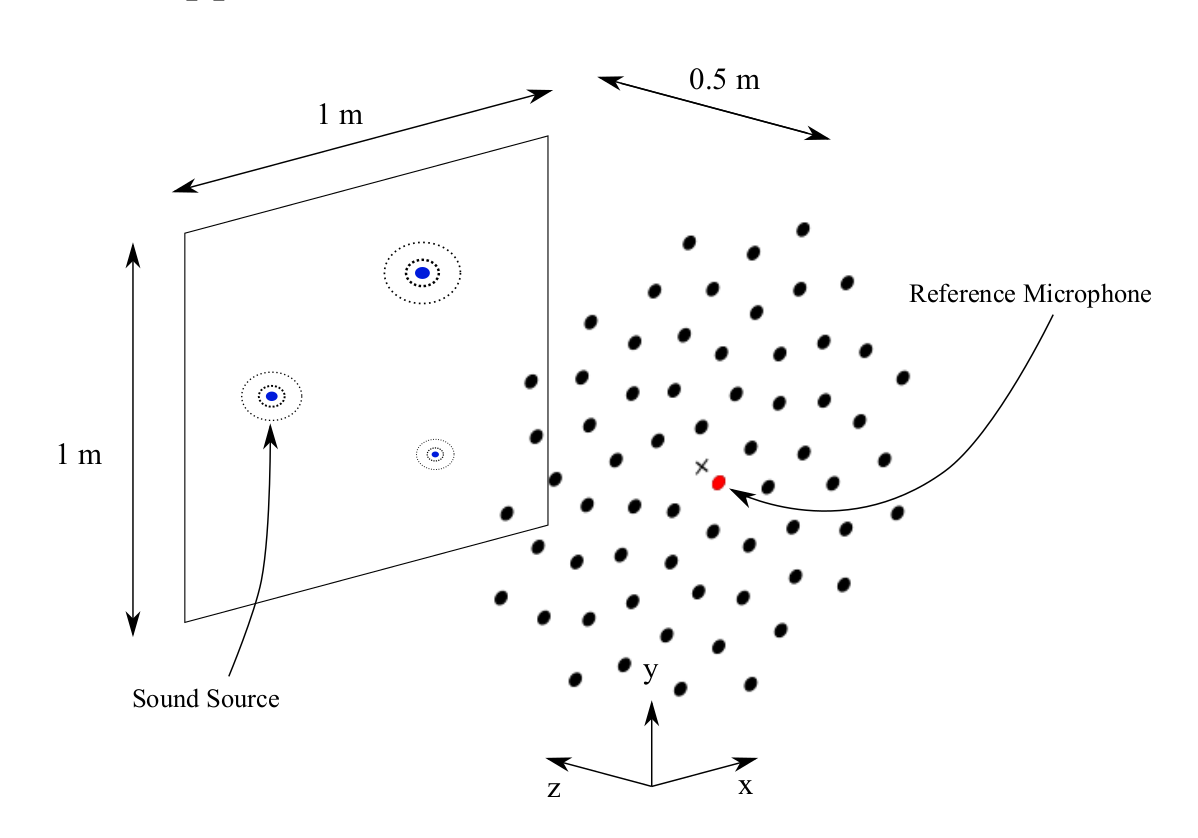
\includegraphics[width=0.65\textwidth]{../figs/full_measurement_setup.png}
    \caption{Example of the measurement setup used, with three audio sources}
    \label{fig:full_measurement_setup}
\end{figure} 

\begin{figure}
    \centering
    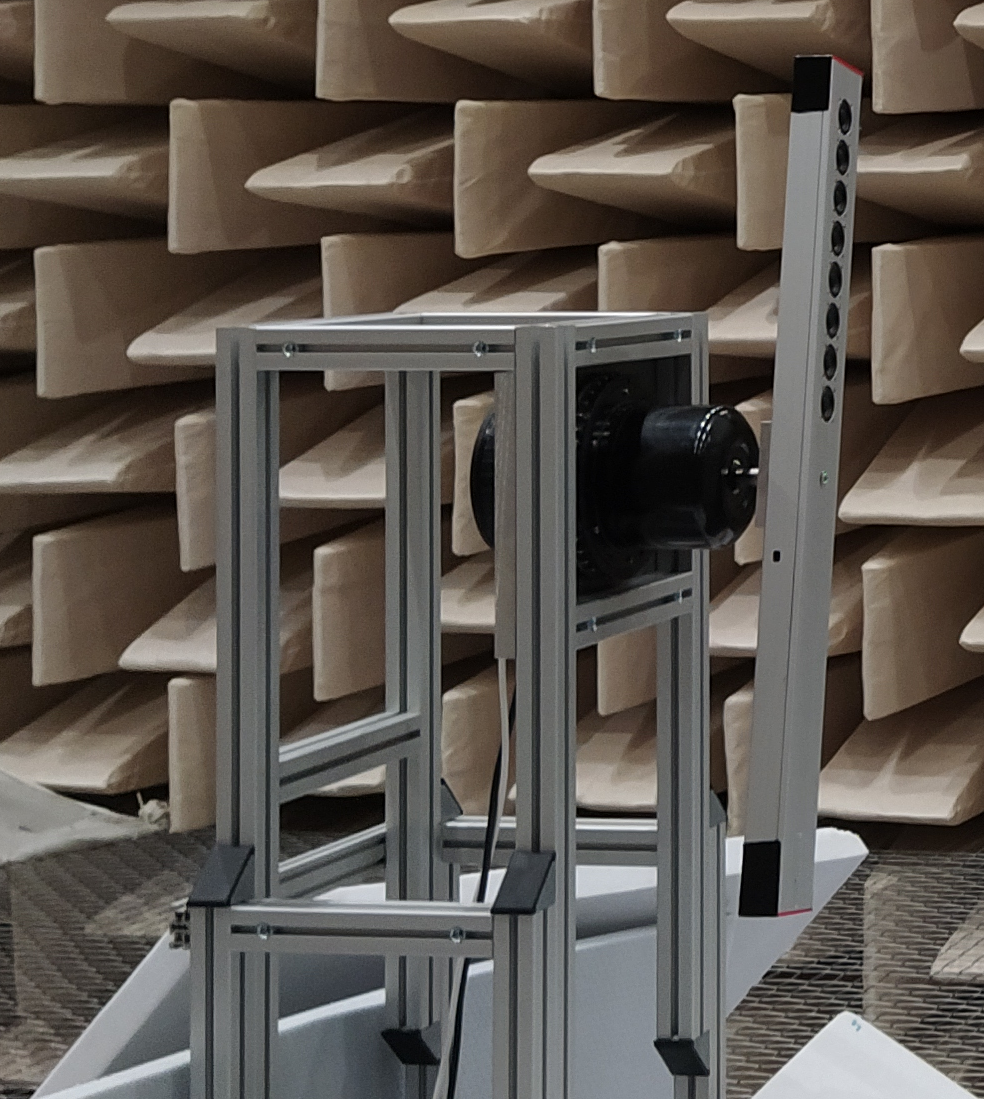
\includegraphics[width=0.65\textwidth]{../figs/source.png}
    \caption{Device used as audio source to create the measurement}
    \label{fig:source}
\end{figure}

\begin{figure}
    \centering
    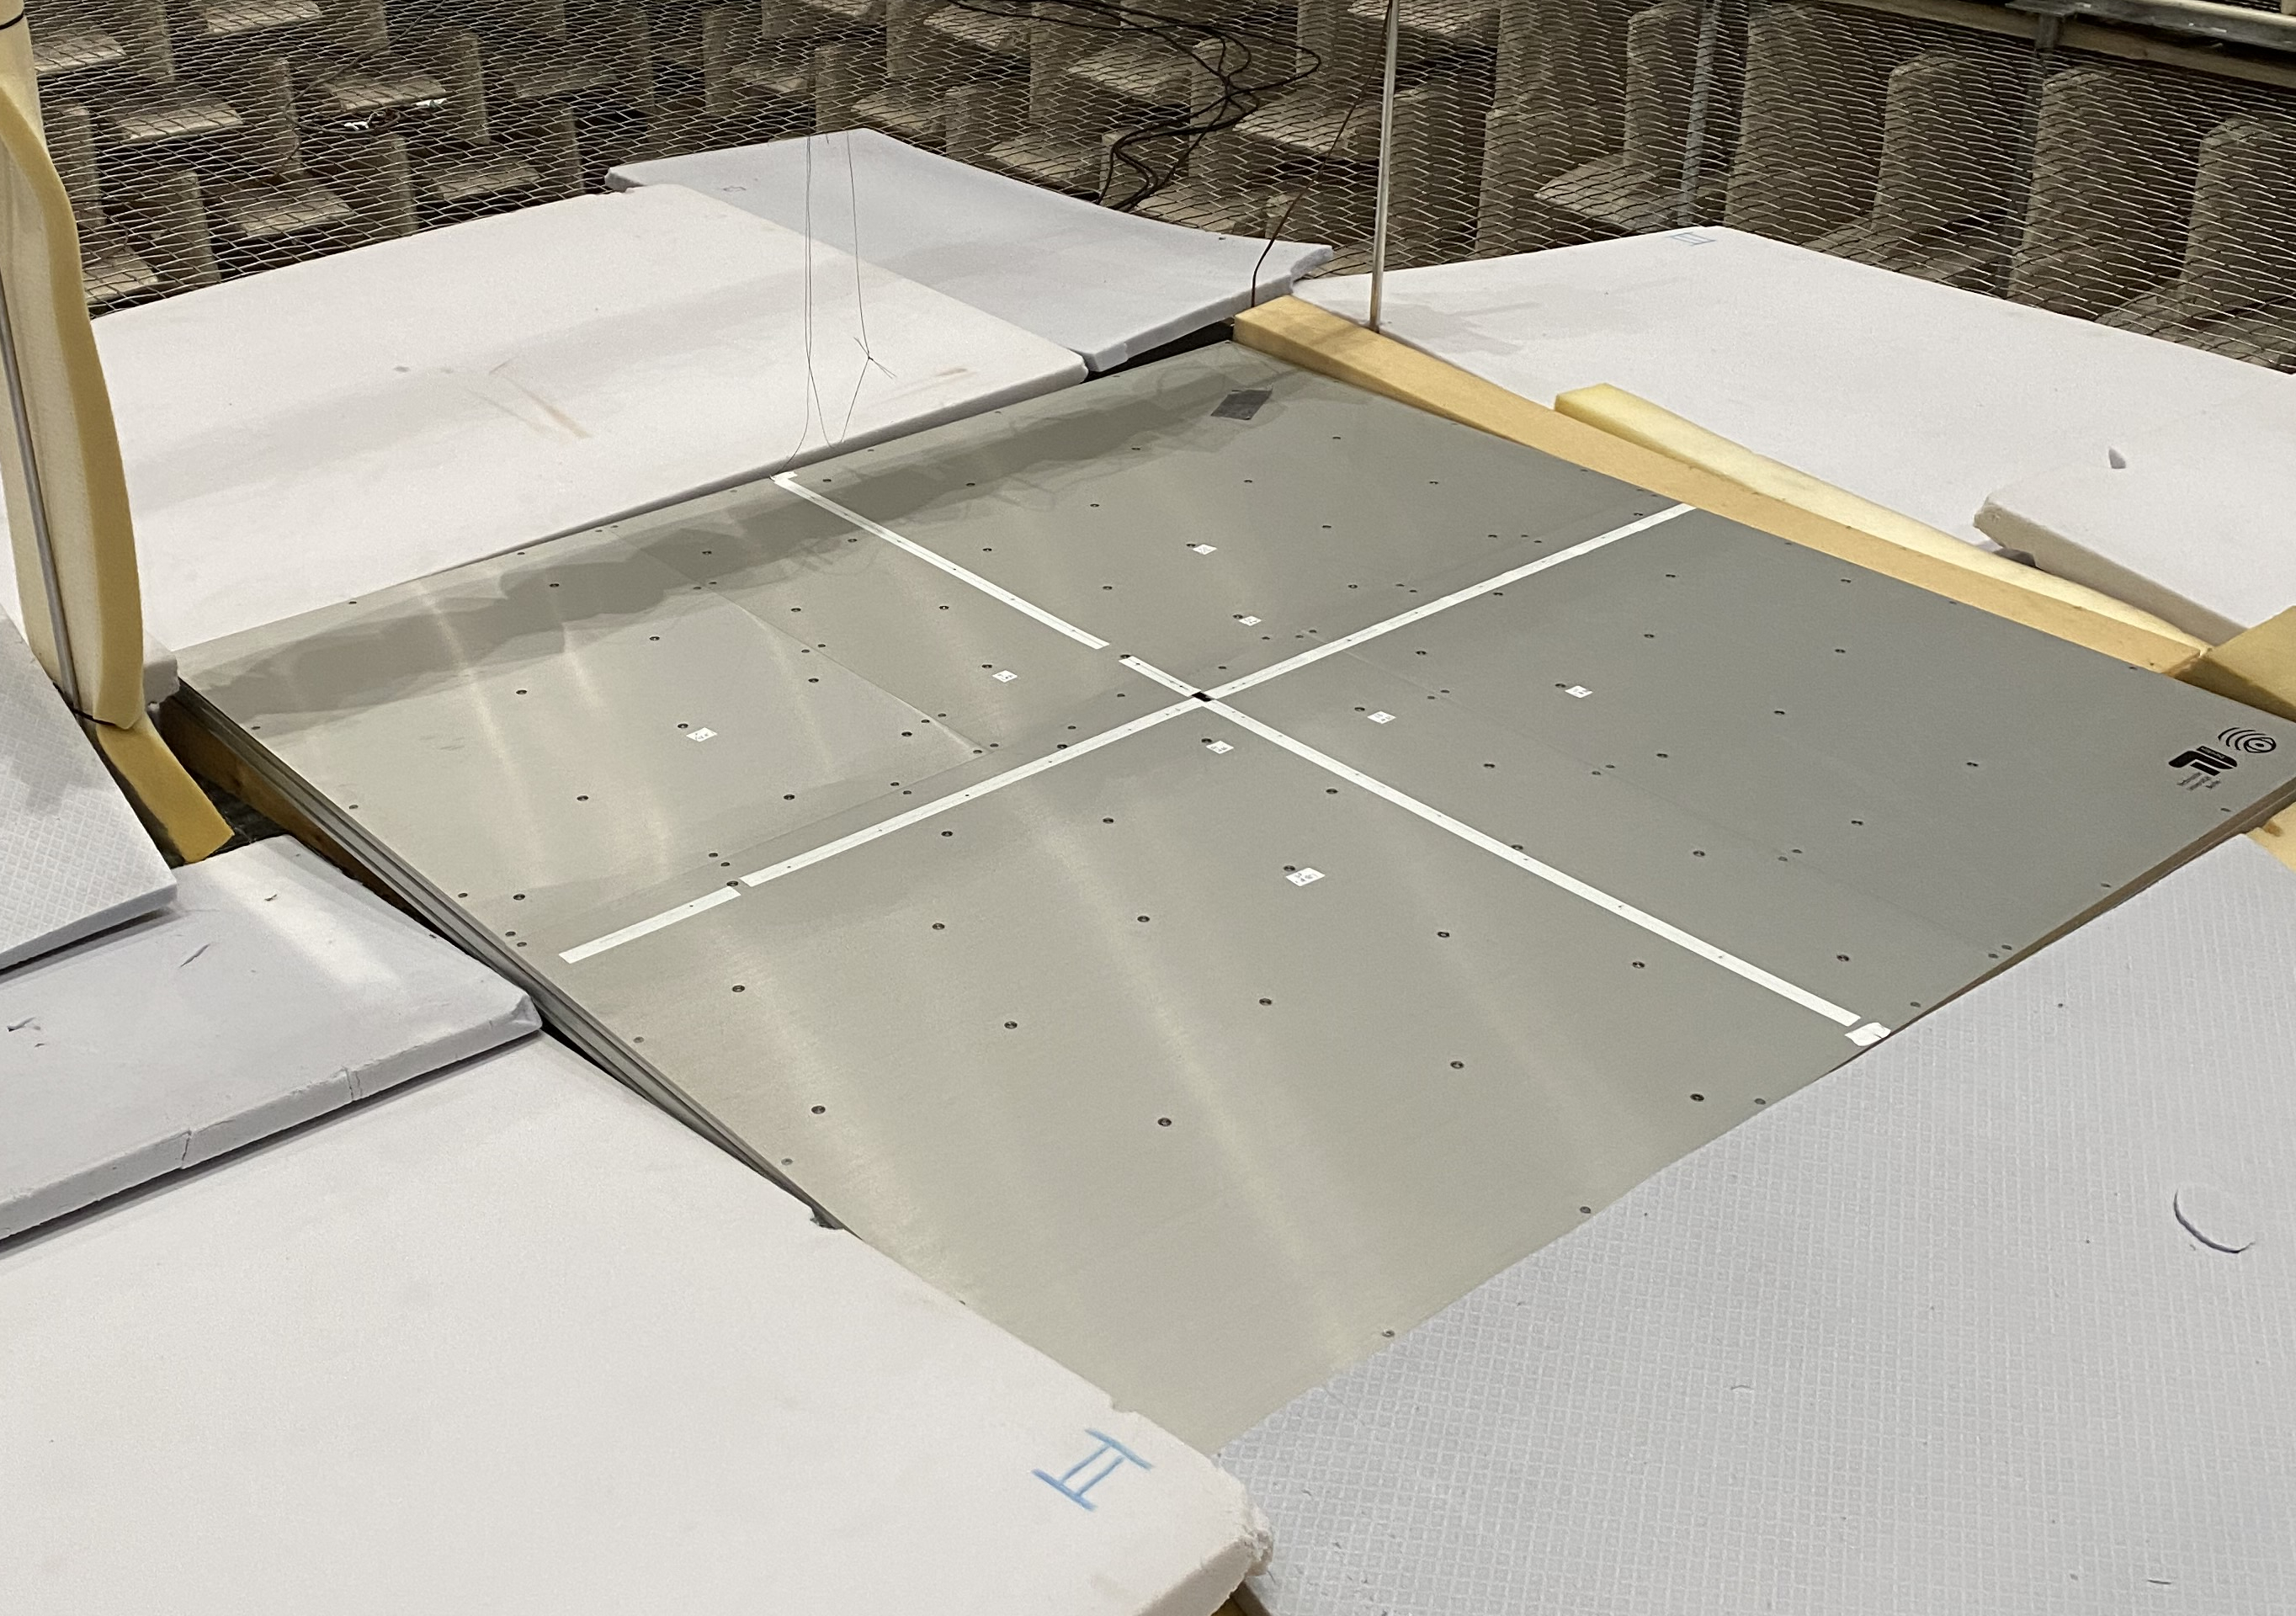
\includegraphics[width=0.65\textwidth]{../figs/microphone_array_cropped.jpg}
    \caption{Picture of the array of microphone used to create the real measurement}
    \label{fig:microphone_array}
\end{figure}    





\subsection{Generation of Eigenvalues}

\subsubsection{WGAN-GP}

In order to generate the eigenvalue, a WGAN-GP was built. The implementation was adapted from \cite{nain2020wgangp}. The data to generate was the eigenvaluess of the CSM. The dimension of the CSM are $64 \times 64$, hence there are 64 eigenvalues to generate.

\subsubsection{Networks Architecture}

As mentionned in the fundamentals the basic structure is two competing networks, a generator and a discriminator or critic. Both architectures of the generator and critic are illustrated respectively in tables Tab.\ref{tab:evals_generator_WGANGP_architecture} and Tab..\ref{tab:evals_critic_WGANGP_architecture}.

Unlike in the implementation of \cite{nain2020wgangp}, both inner networks (generator and critic) do not have a convolutional but a perceptron structure. Indeed, a convolutional structure is relevant when the data to generate is an image. A convolutional layer is good at seeing patterns in image, by identifying structure in batches of neighbour pixels. We could have stacked pieces of our vector of eigenvalues of size 64 into an image of dimesion $8 \times 8$ but this would have resulted in an image where most neighbour pixel are not sharing any information about each other, hence making the convolutional operation irrelevant at detecting pattern, at least compared to images.

Another changes that was made compared to the implementation of \cite{nain2020wgangp}, is that a ReLU actvation function was added as the last layer of the generator. Indeed before this change our generator would generate eigenvalues slightly smaller than zero (of order -1e-10 \textbf{TODO: check actual value}). Moreover, we added 1e-10 to every eigenvalue produced to ensure that they are positive.


\begin{table}[]
    \begin{tabular}{|l|l|l|}
    \hline
    \textbf{Layer}      & \textbf{Output Shape} & \textbf{\#Param.} \\ \hline
    InputLayer          & (None, 128)           & 0                             \\ \hline
    Dense               & (None, 1024)          & 131072                        \\ \hline
    Batch Normalization & (None, 1024)          & 4096                          \\ \hline
    LeakyReLU           & (None, 1024)          & 0                             \\ \hline
    Reshape             & (None, 4, 4, 64)      & 0                             \\ \hline
    UpSampling2D        & (None, 8, 8, 64)      & 0                             \\ \hline
    Conv2D              & (None, 8, 8, 128)     & 73728                         \\ \hline
    BatchNormalization  & (None, 8, 8, 128)     & 512                           \\ \hline
    LeakyReLU           & (None, 8, 8, 128)     & 0                             \\ \hline
    UpSampling2D        & (None, 16, 16, 128)   & 0                             \\ \hline
    Conv2D              & (None, 16, 16, 64)    & 73728                         \\ \hline
    BatchNormalization  & (None, 16, 16, 64)    & 256                           \\ \hline
    LeakyReLU           & (None, 16, 16, 64)    & 0                             \\ \hline
    UpSampling2D        & (None, 32, 32, 64)    & 0                             \\ \hline
    Conv2D              & (None, 8, 8, 1)       & 576                           \\ \hline
    BatchNormalization  & (None, 8, 8, 1)       & 4                             \\ \hline
    Activation          & (None, 8, 8, 1)       & 0                             \\ \hline
    \end{tabular}
    \caption{Architecture of the generator used in the WGAN-GP to generate eigenvalues. Total params: 283,972, Trainable params: 281,538, Non-trainable params: 2,434}
    \label{tab:evals_generator_WGANGP_architecture}
\end{table}



\begin{table}[]
    \begin{tabular}{|l|l|l|}
    \hline
    \textbf{Layer} & \textbf{Output Shape} & \textbf{\#Param.} \\ \hline
    InputLayer     & (None, 8, 8, 1)       & 0                 \\ \hline
    ZeroPadding2D  & (None, 12, 12, 1)     & 0                 \\ \hline
    Conv2D         & (None, 6, 6, 64)      & 1664              \\ \hline
    LeakyReLU      & (None, 6, 6, 64)      & 0                 \\ \hline
    Conv2D         & (None, 3, 3, 128)     & 204928            \\ \hline
    LeakyReLU      & (None, 3, 3, 128)     & 0                 \\ \hline
    Dropout        & (None, 3, 3, 128)     & 0                 \\ \hline
    Conv2D         & (None, 2, 2, 256)     & 819456            \\ \hline
    LeakyReLU      & (None, 2, 2, 256)     & 0                 \\ \hline
    Dropout        & (None, 2, 2, 256)     & 0                 \\ \hline
    Conv2D         & (None, 1, 1, 512)     & 3277312           \\ \hline
    LeakyReLU      & (None, 1, 1, 512)     & 0                 \\ \hline
    Flatten        & (None, 512)           & 0                 \\ \hline
    Dropout        & (None, 512)           & 0                 \\ \hline
    Dense          & (None, 1)             & 513               \\ \hline                               
    \end{tabular}
    \caption{Architecture of the critic used in the WGAN-GP to generate eigenvalues. Total params: 4,303,873, Trainable params: 4,303,873, Non-trainable params: 0}
    \label{tab:evals_critic_WGANGP_architecture}
\end{table}


Finally, before being fed to the discriminator, real and generated eigenvalues are scaled such that the biggest eigenvalue is equal to one. Normalizing eigenvalues in this way is done to reduce the size of the sample space. This is illustrated in Fig.1\ref{fig:evals_wgangp_full_structure}.

\begin{figure}
    \centering
    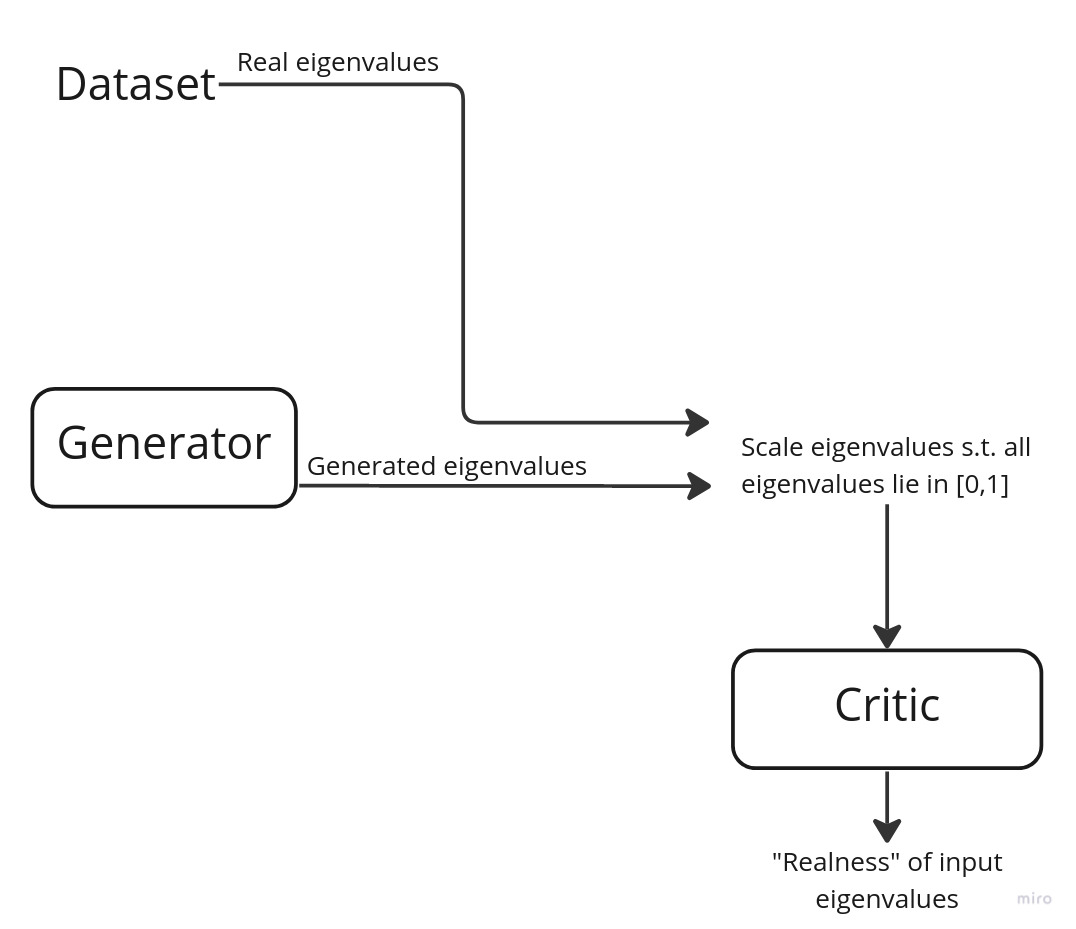
\includegraphics[width=0.65\textwidth]{../figs/evals_wgangp_full_structure.jpg}
    \caption{Full structure of the used implementation of the WGAN-GP to generate eigenvalues.}
    \label{fig:evals_wgangp_full_structure}
\end{figure}

\subsubsection{Performance}

A problem with regular GANs is that it is really hard to know when a good model has been found, from looking only at the loss function. The quality of a model is typically assessed by visually looking at the generated sample and deciding if they are realistic or not. But \cite{arjovsky2017wasserstein} shows that in a WGAN, the loss function of the generator is directly correlated with the quality of the sample produced. This is not true in a regular GAN and is actually one of the main selling point of a WGAN over GAN. With this knowledge, we can observe from the loss function of the generator showed in Fig.\ref{fig:evals_g_loss} actually shows convergence. 

\begin{figure}
    \centering
    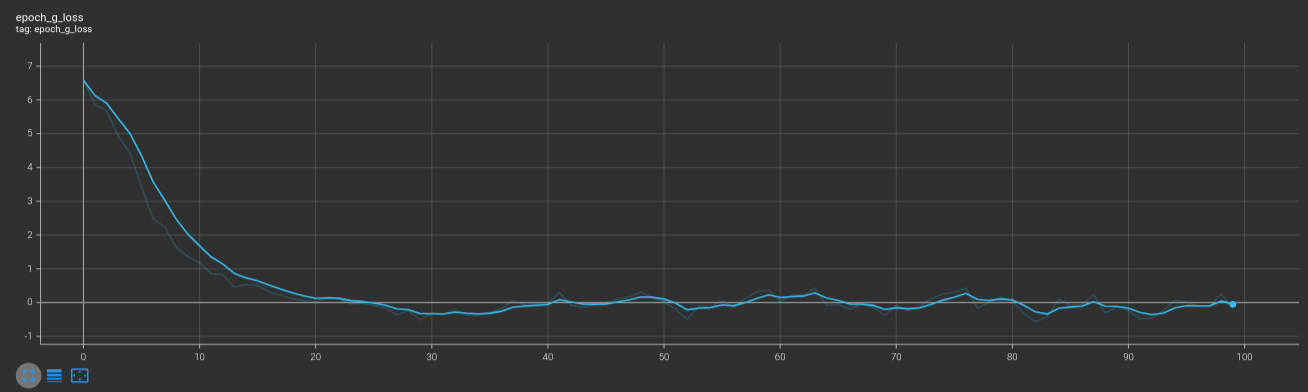
\includegraphics[width=0.9\textwidth]{../figs/evals_g_loss.png}    
    \caption{The loss function of the generator while training the WGAN-GP for eigenvalues generation.}
    \label{fig:evals_g_loss}
\end{figure} 



Moreover when comparing real  and generated eigenvalues sample in Fig.\ref{fig:real_vs_generated_evals}, it can be observed that our WGAN-GP produces sufficiently realisitic results. 

\begin{figure}
    \centering
    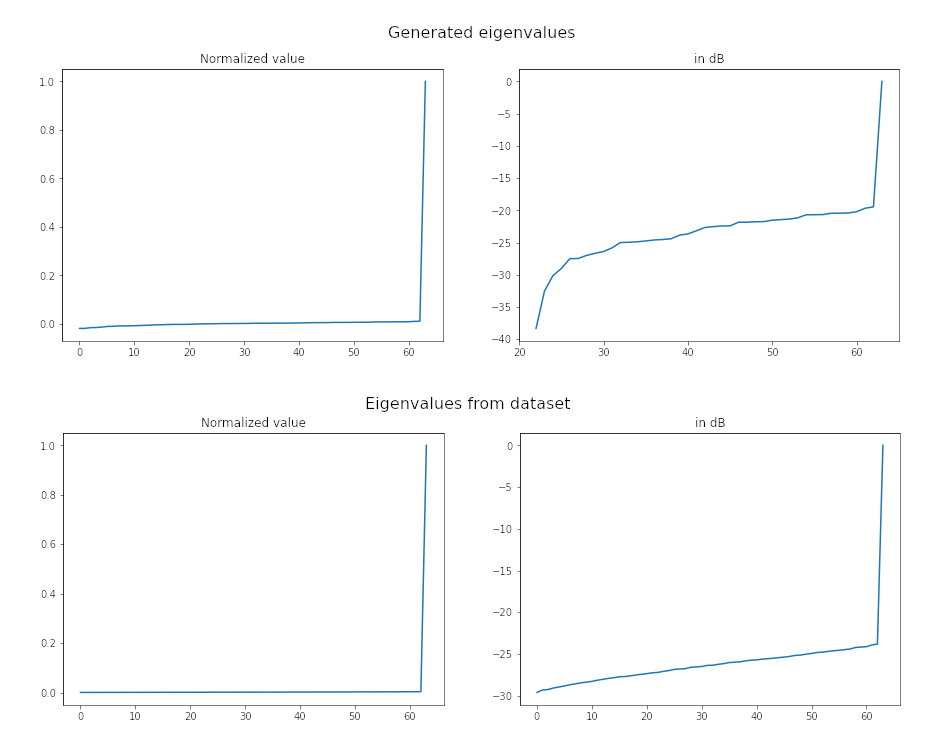
\includegraphics[width=0.9\textwidth]{../figs/real_vs_generated_evals.png}    
    \caption{Top row shows eigenvalues generated by the WGAN-GP, respectively in normal values, followed by their representation in dB. The second shows the same for real eigenvalues.
    }
    \label{fig:real_vs_generated_evals}
\end{figure}

\subsubsection{Generating eigenvalues from their spectrum}

As seen above, the WGAN-GP create convincing spectrum, until they are displayed as level. This led to idea of generating the spectrum from its levels values. We remind here how the level of the eigenvalues $[\lambda_0, \dots, \lambda_{63}] \in \Lambda$ are computed:

\begin{equation}
    L_{\lambda_i} = 10 \log_{10}(\frac{\lambda_i}{\lambda_0})
\end{equation}

where $\lambda_0$ is the biggest eigenvalue. The WGAN-GP used to produce the eigenvalues needed to be adpated in order to produce the level of the spectrum. The architecures  used for the critic and the generator are shown respectively in \textbf{TODO: add new architecture}.

\textbf{TODO: finish writing this part when evals dB is working better}


\subsection{Generation of Eigenvectors}

\subsubsection{WGAN-GP}

The eigenvectors of the cross spectral were generated using two different GANs. The idea behind this not all vectors are sampled from the same distribution. Indeed there is only one main eigenvector (corresponding to a single DoA/source) and 63 "noise" vectors.  Each eigenvector belongs to a different source and all are incoherent. If there would to be  multiple coherent source, all the energy and their position merges into a single eigenmode. The main eigenvector is the one corresponding to the highest eigenvalues. Formally, the set of of all eigenvectors $\mathbf{V} \in \mathbb{C}^{64 \times 64}$ can be divided into two subsets $\mathbf{V}_{\text{main}} \in \mathbb{C}^{64 \times 1}$ and $\mathbf{V}_{\text{noise}} \in \mathbb{C}^{64 \times 63}$, with:

\begin{align}
    v &\sim \mathbb{P}_{\text{main}}  v \in  \mathbf{V}_{\text{main}}\\
    v &\sim \mathbb{P}_{\text{noise}}  v \in  \mathbf{V}_{\text{noise}}
\end{align}
 



% ========================================================================
from mail:
Yes, that makes sense. This  means that the information of multiple DOAs is included in a single eigenvector. Thus, as long as we are dealing with incoherent sources, your remark fully applies.


% ========================================================================


Similarly as for generating the eigenvalues, the eigenvectors were generated using a WGAN-GP whose implementation was adapted from \cite{nain2020wgangp}. There were 64 vectors to generate all of size 64. The vector were stacked in a matrix such that the data to generate was an image of dimension $64 \times 64$.



\subsubsection{Architecture}

Again, we have two networks forming the WGAN-GP: a generator and a discriminator or critic. The architectures of both the generator and critic are illustrated respectively in the tables Tab.\ref{tab:evecs_generator_WGANGP_architecture} and Tab.\ref{tab:evecs_critic_WGANGP_architecture}. Similarily as for the eigenvalues, the architectures used are directly adapted from \cite{nain2020wgangp} in order to produce data with desired dimensions.



\begin{table}[]
    \begin{tabular}{|l|l|l|}
    \hline
    \textbf{Layer}      & \textbf{Output Shape} & \textbf{\#Param.} \\ \hline
    InputLayer          & (None, 128)           & 0                 \\ \hline
    Dense               & (None, 16384)         & 2097152           \\ \hline
    Batch Normalization & (None, 16384)         & 65536             \\ \hline
    LeakyReLU           & (None, 16384)         & 0                 \\ \hline
    Reshape             & (None, 8, 8, 256)     & 0                 \\ \hline
    UpSampling2D        & (None, 16, 16, 256)   & 0                 \\ \hline
    Conv2D              & (None, 16, 16, 128)   & 294912            \\ \hline
    Batch Normalization & (None, 16, 16, 128)   & 512               \\ \hline
    LeakyReLU           & (None, 16, 16, 128)   & 0                 \\ \hline
    UpSampling2D        & (None, 32, 32, 128)   & 0                 \\ \hline
    Conv2D              & (None, 32, 32, 64)    & 73728             \\ \hline
    Batch Normalization & (None, 32, 32, 64)    & 256               \\ \hline
    LeakyReLU           & (None, 32, 32, 64)    & 0                 \\ \hline
    UpSampling2D        & (None, 64, 64, 64)    & 0                 \\ \hline
    Conv2D              & (None, 64, 64, 1)     & 576               \\ \hline
    Batch Normalization & (None, 64, 64, 1)     & 4                 \\ \hline
    Activation          & (None, 64, 64, 1)     & 0                 \\ \hline
    \end{tabular}
    \caption{Architecture of the generator used in the WGAN-GP to generate eigenvectors. Total params: 2,532,676, Trainable params: 2,499,522, Non-trainable params: 33,154}
    \label{tab:evecs_generator_WGANGP_architecture}
\end{table}

\begin{table}[]
    \begin{tabular}{|l|l|l|}
    \hline
    \textbf{Layer} & \textbf{Output Shape} & \textbf{\#Param.} \\ \hline
    InputLayer     & (None, 64, 64, 2)     & 0                 \\ \hline
    ZeroPadding    & (None, 68, 68, 2)     & 0                 \\ \hline
    Conv2D         & (None, 34, 34, 64)    & 3264              \\ \hline
    LeakyReLU      & (None, 34, 34, 64)    & 0                 \\ \hline
    Conv2D         & (None, 17, 17, 128)   & 204928            \\ \hline
    LeakyReLU      & (None, 17, 17, 128)   & 0                 \\ \hline
    Dropout        & (None, 17, 17, 128)   & 0                 \\ \hline
    Conv2D         & (None, 9, 9, 256)     & 819456            \\ \hline
    LeakyReLU      & (None, 9, 9, 256)     & 0                 \\ \hline
    Dropout        & (None, 9, 9, 256)     & 0                 \\ \hline
    Conv2D         & (None, 5, 5, 512)     & 3277312           \\ \hline
    LeakyReLU      & (None, 5, 5, 512)     & 0                 \\ \hline
    Flatten        & (None, 12800)         & 0                 \\ \hline
    Dropout        & (None, 12800)         & 0                 \\ \hline
    Dense          & (None, 1)             & 12801             \\ \hline
    \end{tabular}
    \caption{Architecture of the critic used in the WGAN-GP to generate eigenvectors. Total params: 4,317,761, Trainable params: 4,317,761, Non-trainable params: 0}
    \label{tab:evecs_critic_WGANGP_architecture}
\end{table}



In order to reduce the sample space, both the real and generated eigenvectors are normalized before being fed to the discriminator. The full WGAN-GP structure is illutrates in Fig.\ref{fig:evecs_wgangp_full_structure}.


\begin{figure}
    \centering
    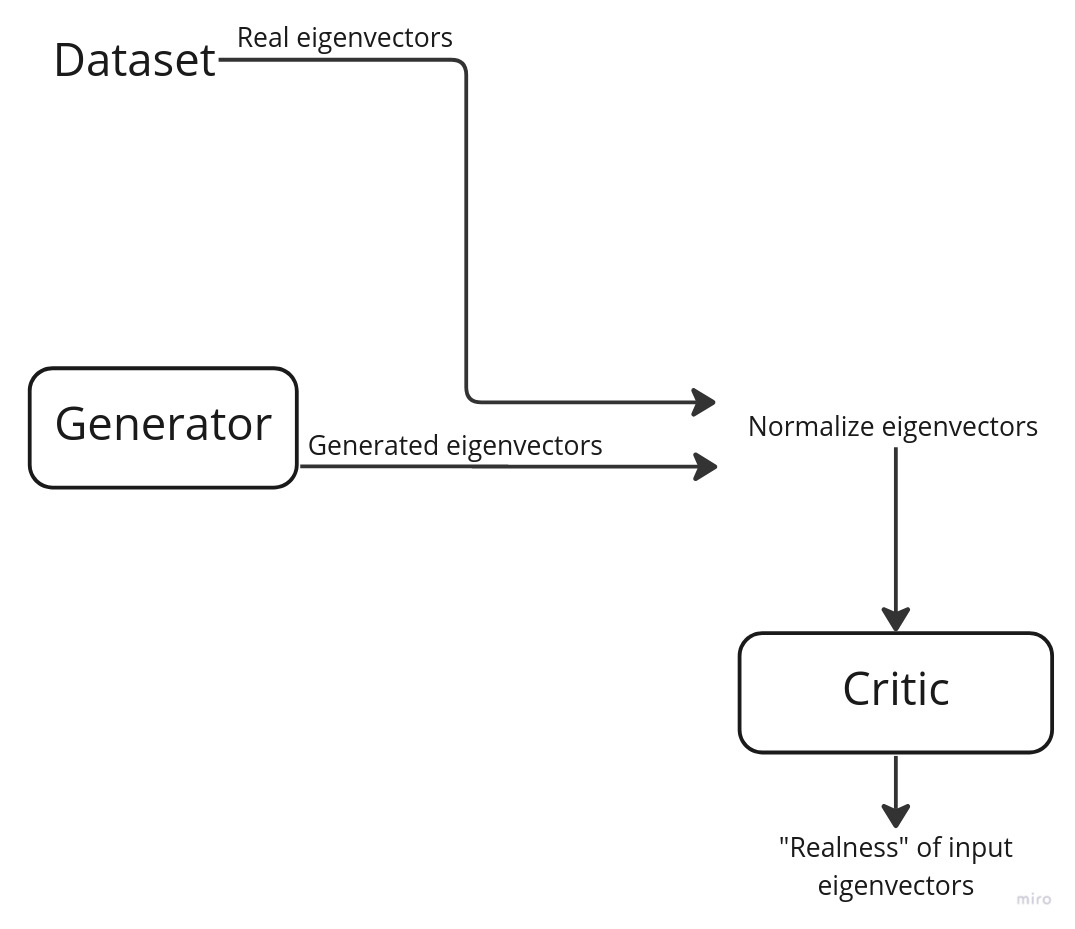
\includegraphics[width=0.65\textwidth]{../figs/evecs_wgangp_full_structure.jpg}
    \caption{Full structure of the used implementation of the WGAN-GP to generate eigenvectors.}
    \label{fig:evecs_wgangp_full_structure}
\end{figure}

\subsubsection{Performance} 



\subsection{Data Augmentation}

As seen before, we have some quite realistic looking generated eigenvalues. This led to the following idea for increasing the number of training samples (data augmentation). First, for a set of received CSM, decompose them in eigenvalues $\mathbf{\Lambda}$  and eigenvectors $\mathbf{V} = [\mathbf{v}_1^T, \dots, \mathbf{v}_M^T]$ with:

\begin{equation}
    \mathbf{\hat{C}} = \mathbf{V} \mathbf{\Lambda} \mathbf{V}^H
\end{equation}


The set of all eigenvalues can then be used to train a WGAN-GP. Using this network, we can generated eigenvalues $\hat{\mathbf{\Lambda}}$, which are realistic, up to an unknown scaling factor $c \in \mathbb{R}$.  


Then using the generated eigenvalues $\hat{\mathbf{\Lambda}}$ with real eigenvectors $\mathbf{V}$ we can have semi-generated CSM:

\begin{equation}
    \mathbf{\hat{C}}_\text{augm.}  = \mathbf{V} \hat{\mathbf{\Lambda}} \mathbf{V}^H
\end{equation}

which are realistic up to the scaling factor $c$. \textbf{TODO: show that the scaling factor $c$ does influence the beamforming}.

\subsubsection{Comparison between augmented data and real data.}


Fig.\ref{fig:beamforming_real_csm} and Fig.\ref{fig:beamforming_augmented_csm} show respectively the result of performing beamforming on a real CSM issued from the dataset and from a semi generated CSM. Both CSM have been recreated from the eigenvalue decomposition. It can be observed that both results are visually similar. A more careful obserbartion allows to notice that despite looking similar proportinaly, the overall values of in the beamforming map resulting from real data are slightly higher. This is due to the scaling of the eigenvalues taking place in the generative process. 

\begin{figure}
    \centering
    \begin{minipage}{0.45\textwidth}
        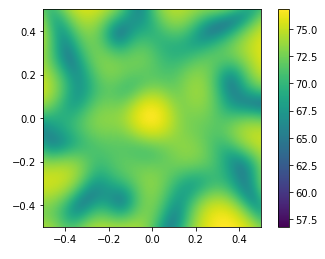
\includegraphics[width=1.2\textwidth]{../figs/beamforming_real_csm.png}
        \caption{Results of beamforming from a real CSM}
        \label{fig:beamforming_real_csm}
    \end{minipage}\hfill
    \begin{minipage}{0.45\textwidth}
        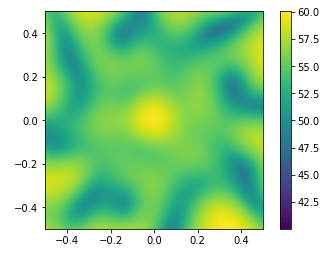
\includegraphics[width=1.2\textwidth]{../figs/beamforming_augmented_csm.png}
        \caption{Results of beamforming from a CSM issued from augmented data}
        \label{fig:beamforming_augmented_csm}
    \end{minipage}
\end{figure}

\subsection{Generation of Cross-Correlation Matrix}
% ========================================================================


\section{Future work}

\textbf{TODO}: here need to mention TransGAN, need to mention that the GAN could be made conditional 

% Bibliography
% Cite: version 1
%\printbibliography

 

% Cite: version 2
\bibliography{../mybib}
\bibliographystyle{plainnat}

\end{document}